\chapter{Outer Tracker Luminometer}

The CMS Phase II Outer Tracker  (OT) system will provide a source of high rate physics objects: L1 track stubs.
In its designed architecture these objects are sent to the L1 track reconstruction system at full 40 MHz frequency~\cite{CERN-LHCC-2017-009}.
Studies of CMS Phase II simulations show excellent linearity in the counting of these objects up to pile-up of 200.
These properties make this an excellent candidate for a precision luminometer.
In the following sections the detector layout, a preliminary design of the data acquisition system, and the expected perfomace are described.


\section{Detector Layout and track stub reconstruction}

The design of the Phase II OT is described in Chapter 3 of The Phase-2 Upgrade of the CMS Tracker TDR ~\cite{CERN-LHCC-2017-009} and shown below in Figure~\ref{fig:OT_layout}.
The layout consists of 6 barrel layers (3 TBPS + 3 TB2S) and 5 endcap (TEDD) disks.
The design of the CMS Phase II L1 trigger system requires the reconstruction of track stubs in the front-end of the OT in order to aid the track reconstruction for the L1 trigger.
For the luminosity measurement, CMS detector simulations have been studied up to the Phase II expected pile-up,
these studies described below show that the best precision can be obtained with the track stub counting from the barrel layer 6. 
The OT barrel layer 6 consists of 78 ladders on each side of the detector, with each ladder containing 12 sensor modules as shown in Figure~\ref{fig:OT_ladder_stub}.
The track stub reconstruction (right side of Figure ~\ref{fig:OT_ladder_stub}) is performed with firmware algorithms in the front-end electronics and transmitted to the back-end for all LHC bunch crossings.


\begin{figure}[hbtp]
\centering
\begin{subfigure}
\centering
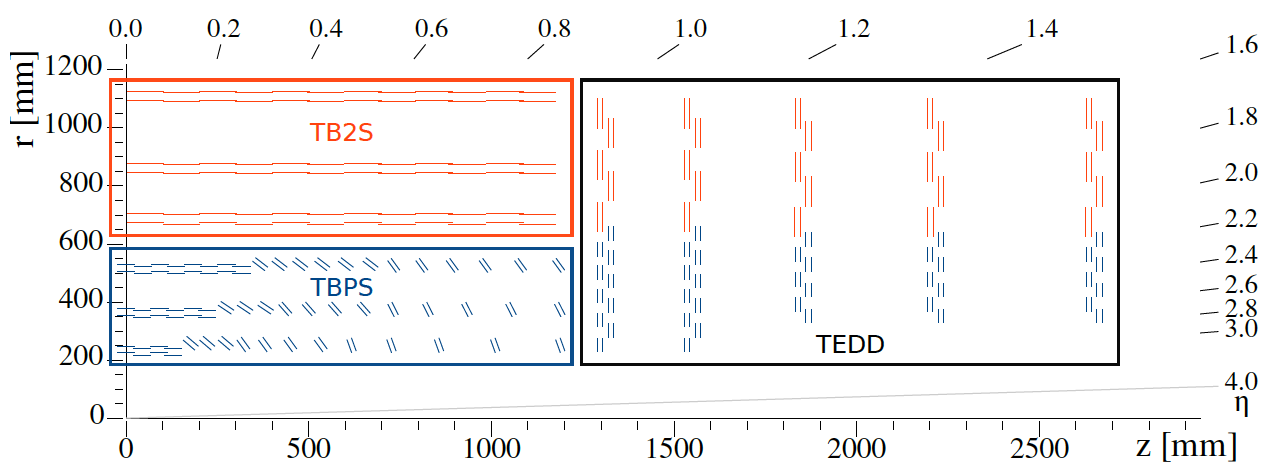
\includegraphics[width=.9\linewidth]{tex/Part2/fig/OT/OT-longitudinal.png}
\end{subfigure}
\caption{
  Longitudinal view of the CMS Phase II Outer Tracker layout  with two regions in the barrel (TB2S, TBPS) and the endcap region (TEDD).
  For the luminosity measurement only the barrel outermost layer 6 in the TB2S part is used, this layer consists of 78 sensor ladders on each side of CMS.
}
\label{fig:OT_layout}
\end{figure}


\section{Data Acquisition}

A design of the OT DAQ including both the front-end and back-end systems is shown in Figure~\ref{fig:OT_DAQ}.
The back-end consists of Data, Trigger, and Control (DTC) boards which process the Trigger (TRIG) stream containting the track stub information. 
The list of track stubs reconstructed for each bunch crossing is transmitted in blocks of 8 bunch crossings to the DTC boards.
For the luminosity measurement, a specialized {\it BRIL Histogramming} firmware module has been developed which will count the number of track stubs in each bunch crossing and produce a histogram per orbit (3654 bunch crossings) at regular integration intervals of 1 second.

Each luminosity histogram will be configured to integrate track stubs from one 12 module ladder, the DTC boards process 3-6 ladders.
The number of necessary instances of  {\it BRIL Histogramming} modules will be installed in the DTC boards and readout via IPBus network protocol to the BRIL-DAQ system for further processing and storage.
Considering the rate of track stubs per ladder estimated with CMS simulations at pile-up of 200  (Figure~\ref{fig:OT_rates}),  the necessary memory per luminosity histogram is estimated using 32-bit memory words as follows: 3564 stub counting words (bins/orbit) + 9 words header + 2 words module mask + 192 error words (12 modules * 8 errors * 2 words/error) for a total of 3767 words per histogram.
In the case of 6 ladders per DTC this corresponds to a data readout rate of ~496 kbps.
For the total of 156 OT histograms, the total data rate received by the BRIL-DAQ is approximately 18.8 Mbps.


\clearpage

\begin{figure}[t]
\centering
\begin{subfigure}
  \centering
  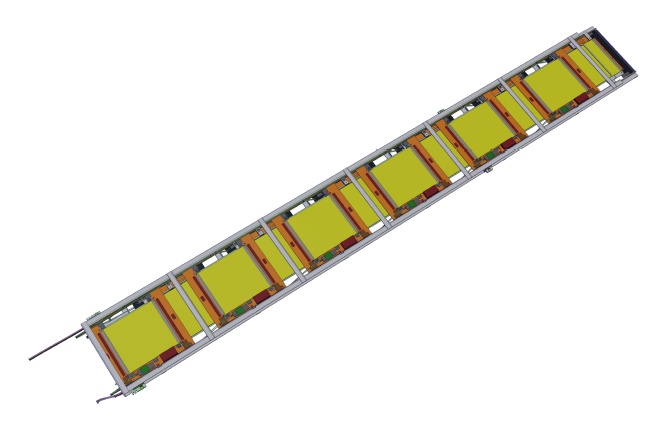
\includegraphics[width=.48\linewidth]{tex/Part2/fig/OT/OT-ladder.png}
\end{subfigure}
\begin{subfigure}
  \centering
  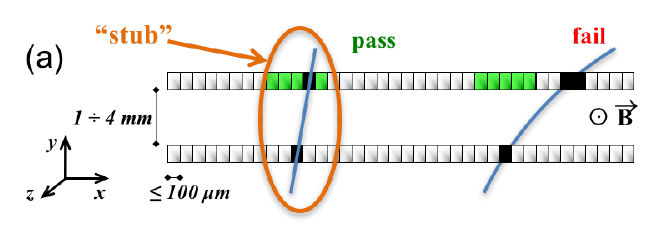
\includegraphics[width=.48\linewidth]{tex/Part2/fig/OT/OT-stub.png}
\end{subfigure}
\caption{
  Layout of one OT sensor ladder with 12 modules (left) and diagram of the track stub reconstruction (right) using the two sensor layers in each module.  
}
\label{fig:OT_ladder_stub}
\end{figure}



\begin{figure}[hbtp]
\centering
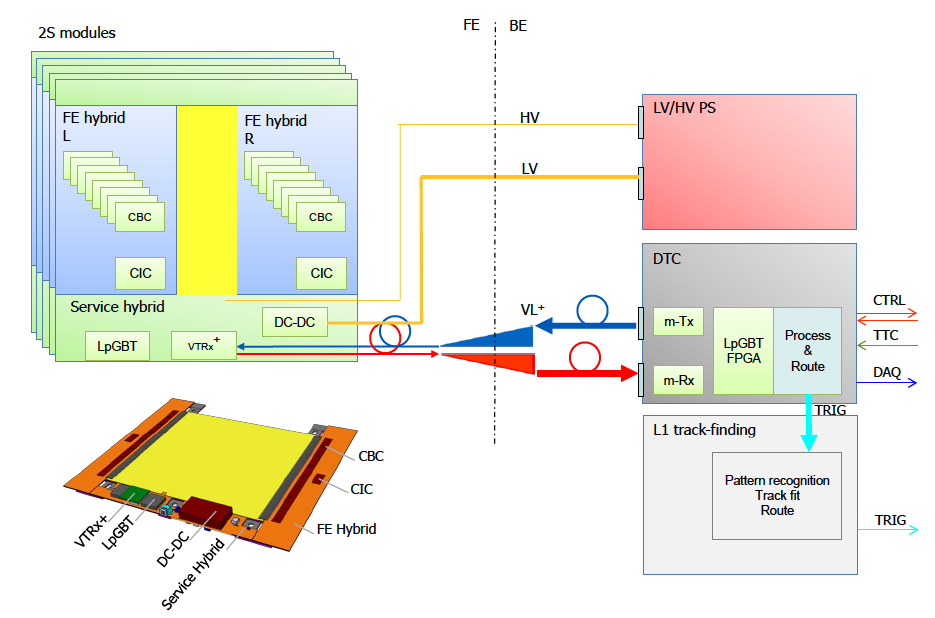
\includegraphics[width=.85\linewidth]{tex/Part2/fig/OT/OT-DAQoverview.png}
\caption{
  Design of the Phase II Outer Tracker frontend (FE) and backend (BE) electronics~\cite{CERN-LHCC-2017-009}.  
}   
\label{fig:OT_DAQ}
\end{figure}


\clearpage

\section{Expected Performance}
%- Rates\\
%- linearity \\
%- statistical precision

The performance of the Phase II OT has been studied using detailed detector simulations for a wide range of pile-up scenarios. The samples have been privately produced using CMSSW version 11\_2\_0\_pre6 and a custom geometry that includes only the tracker volume with geometry versions 6.1.3 and 6.1.6 for the Inner and Outer Tracker, respectively.They also contain simulated effects from front-end electronics, specifically for the OT 2S modules the CBC hit detection mode is set to latched. Similar to what was done for TEPX simulations (see section \ref{sec:TEPX_sim}), the process that has been used to generate these samples is a single-neutrino event overlaid with a variable number of minimum-bias events to simulate pile-up. 

To test the linearity, the number of stubs is histogrammed per event for each layer of the OT. The mean of these distributions is then plotted as a function of pile-up, and a line is fitted to the lowest pile-up points (between 0 and 2) and then extrapolated to higher values, up to a pile-up of 200. Figure \ref{fig:OT_linearity} shows the linearity of stubs for all OT barrel layers. The deviation from a perfectly linear behaviour is presented in figure \ref{fig:OT_deviation}, where it can be seen that layer 6 has a deviation of less than 1\% across the full pile-up range.

\begin{figure}[h!]
\centering
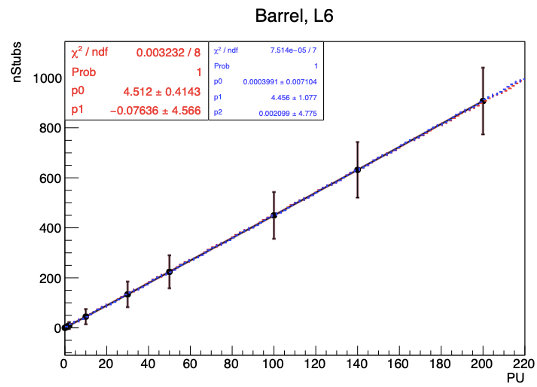
\includegraphics[width=.6\linewidth]{tex/Part2/fig/OT/OT-linearity.png}
\caption{
 Average number of track stubs per event as a function of pile-up determined from the CMS Phase II simulation showing a linear behaviour. \nts{PLACEHOLDER: To be replaced with a linearity plot including all barrel layers.}
} 
\label{fig:OT_linearity}
\end{figure}

\begin{figure}[h!]
\centering
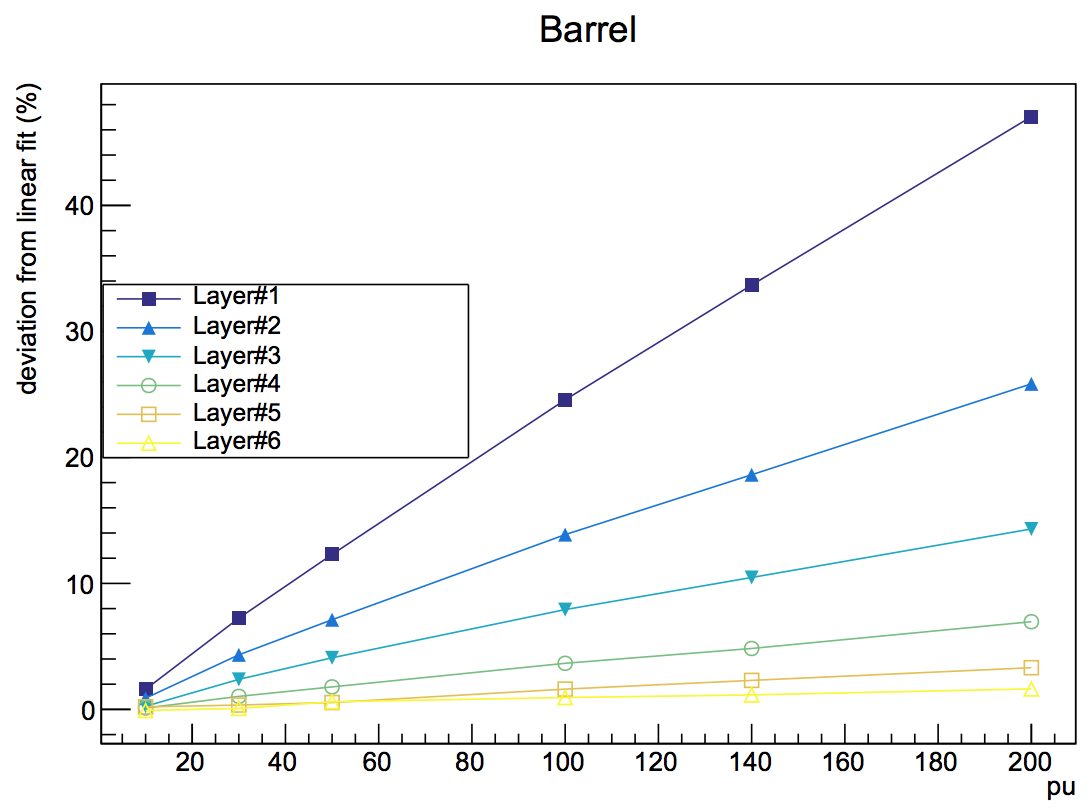
\includegraphics[width=.6\linewidth]{tex/Part2/fig/OT/OT-deviation.png}
\caption{
 Deviation from linearity for all barrel layers of the OT. \nts{PLACEHOLDER: To be replaced with plot using CMS style.}
}
\label{fig:OT_deviation}
\end{figure}

Another important figure of merit for the performance of the OT as a luminometer is the statistical precision that can be achieved. Figure \ref{fig:OT_rates} shows the average number of stubs per event per ladder in layer 6, obtained from the simulations described above. The maximum total rate for the pile-up step of 200 is found to be of 902 stubs per event for Physics and of 2.255 for vdM conditions. With these counts, and considering a trigger readout rate of 40~MHz and an integration period of 1~s (30~s), a statistical precision of 0.03\% (0.115\%) per bunch-crossing is expected for Physics (vdM) conditions.   

\begin{figure}[h!]
\centering
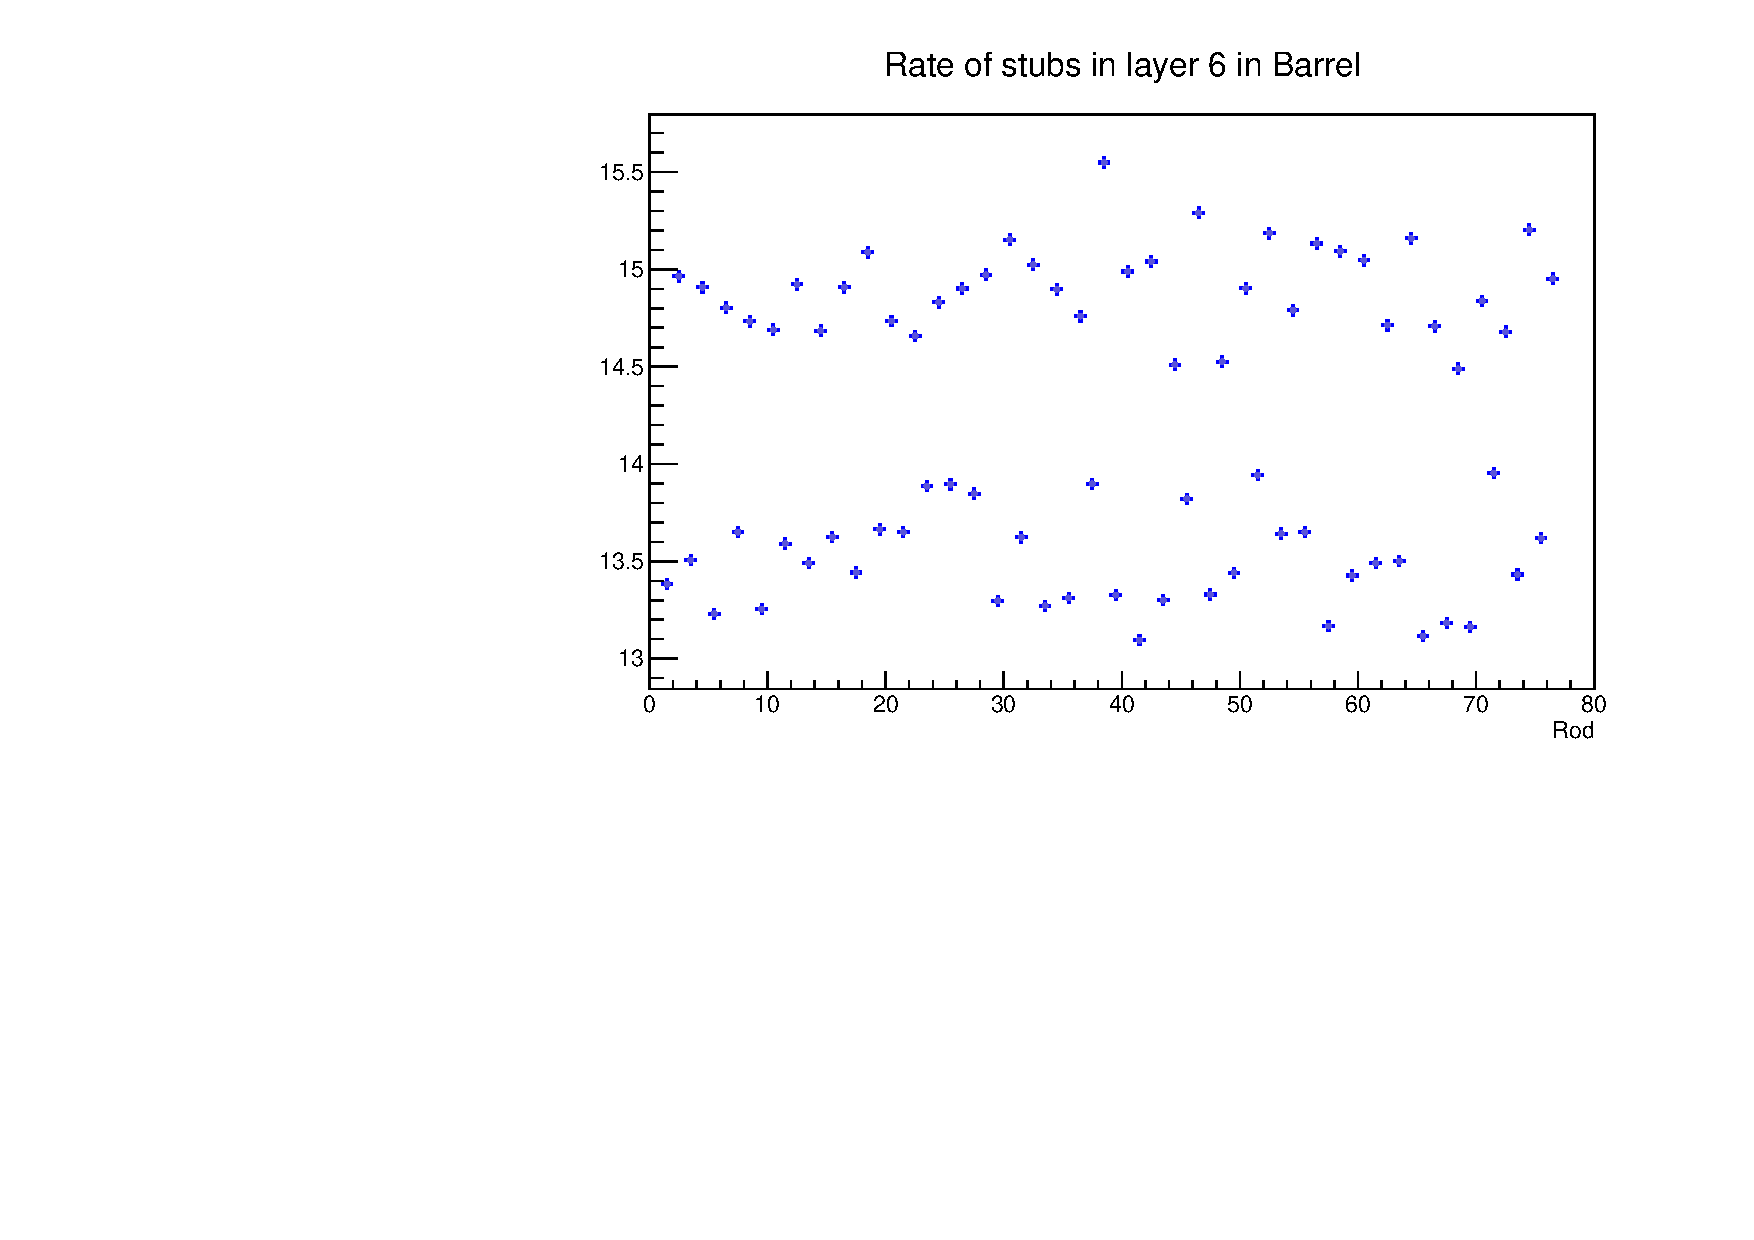
\includegraphics[width=.6\linewidth]{tex/Part2/fig/OT/OT-Rates.pdf}
\caption{
  Average number of track stubs per event per ladder as a function of the ladder id.
  The rate is determined from the CMS Phase II simulation for a pile-up of 200. \nts{PLACEHOLDER: To be replaced with plot using CMS style.}
}
\label{fig:OT_rates}
\end{figure}




